\documentclass[a4paper, 12pt, dvipsnames]{article}
\usepackage[utf8]{inputenc}

%=== Packages ===%

% German language encoding
% \usepackage[ngerman]{babel}
% \usepackage[utf8]{inputenc}
% \usepackage[T1]{fontenc}

% generate dummy text
\usepackage{lipsum}  

% decrease caption size
\usepackage{caption}
\captionsetup{font=footnotesize}

% chess board
\usepackage{xskak}

% multiple footnotes
\usepackage[multiple]{footmisc}

% add graphics
\usepackage{graphicx}

% graphics next to each other
\usepackage{subcaption}

% used for custom enumarations
\usepackage{enumerate}
\usepackage[shortlabels]{enumitem}

% improved tabular package
\usepackage{tabularx}

% for hyperlinks
\usepackage[hidelinks]{hyperref}

% Bibliography/Citations
\usepackage{cite}
\usepackage{natbib}

\usepackage{ifthen}

\usepackage{acronym}

%=== Document Setup ===%

% set margin
% use 2cm at the top if no header is used
% use 2.5cm at the bottom if fotter is used
\usepackage[left=1.5cm, right=1.5cm, top=2.5cm, bottom=1cm]{geometry}

% headline
\usepackage{fancyhdr}
\usepackage{enumitem}
\usepackage{amsmath}
\usepackage{amssymb}

\pagestyle{fancy}
\fancyhf{}
\rhead{Seite \thepage}
\lhead{Diskrete Mathematik}
% \cfoot{}

% for inline code blocks
\usepackage{listings}
\usepackage{xcolor}

\definecolor{backcolour}{RGB}{245, 245, 245}

\lstdefinestyle{codestyle}{
	backgroundcolor=\color{backcolour},
    commentstyle=\color{gray},
    numberstyle=\ttfamily\scriptsize,
    basicstyle=\ttfamily\footnotesize,
    breakatwhitespace=false,         
    breaklines=true,                 
    captionpos=b,                    
    keepspaces=true,                 
    numbers=left,                    
    numbersep=5pt,                  
    showspaces=false,                
    showstringspaces=false,
    showtabs=false,                  
    tabsize=2,
    % xleftmargin=0.15in
}

\lstset{style=codestyle}

\usepackage{parskip}

\usepackage{titlesec}

\titleformat*{\section}{\Large\bfseries}
\titleformat*{\subsection}{\normalsize\bfseries}
\titleformat*{\subsubsection}{\normalsize\bfseries}

\usepackage{multicol}

\usepackage[normalem]{ulem}

\usepackage{mathtools}

\begin{document}

\section{Abzählungen}

Es gibt nur zwei Arten von Aufgaben:

\begin{itemize}
\item Anzahl Aufteilungen von einer Menge $N$ von Kugeln in eine Menge $R$ von Fächern
\item Aus einer Menge $N$ mit $n$ Elementen sollen alle oder $k$ Elemente ausgewählt werden
\end{itemize}

\subsection{Anzahl Aufteilungen von einer Menge $N$ von Kugeln in eine Menge $R$ von Fächern}

\begin{table}[h]
\centering
\begin{tabular}{l|c|l|l|l}
$|N| = n, |R| = r$ & beliebig & injektiv & surjektiv & bijektiv\\
\hline
% === %
$N$ unterscheidbar & & $r \geq n : r^{\underline{n}}$ & $n \geq r : r!S_{n,r}$ & $r = n : n!$\\
$R$ unterscheidbar & $r^n$ & $r < n : 0$ & $n < r : 0$ & $r \neq n : 0$\\
\hline
% === %
$N$ nicht unterscheidbar & $\begin{pmatrix}r + n - 1\\ n\end{pmatrix}$ & $r \geq n : \begin{pmatrix}r\\ n\end{pmatrix}$ & $n \geq r: \begin{pmatrix}n-1\\ r-1\end{pmatrix}$ & $r = n : 1$\\
$R$ unterscheidbar & $\displaystyle = \frac{r^{\overline{n}}}{n!}$ & $r < n : 0$ & $n < r : 0$ & $r \neq n : 0$\\
\hline
% === %
$N$ unterscheidbar & & $r \geq n : 1$ &  $n \geq r : S_{n,r}$ & $r = n : 1$\\
$R$ nicht unterscheidbar & $\displaystyle \sum_{k=1}^{r}S_{n,k}$ & $r < n : 0$ & $n < r : 0$ & $r \neq n : 0$\\
\hline
% === %
$N$ nicht unterscheidbar & & $r \geq n : 1$ & $n \geq r : P_{n,r}$ & $r = n : 1$\\
$R$ nicht unterscheidbar & $\displaystyle \sum_{k=1}^{r} P_{n,k}$ & $r < n : 0$ & $n < r : 0$ & $r \neq n : 0$
\end{tabular}
\end{table}

\textbf{Beliebige Aufteilung:}

\begin{itemize}[leftmargin=*]
\item Keine speziellen Regeln bei der Aufteilung (Man kann die Kugeln verteilen wie man möchte)
\begin{itemize}
\item[$\Rightarrow$] Ein Fach darf leer sein, kann eine Kugel haben oder mehrere Kugeln haben
\end{itemize}
\item Alle Kugeln müssen benutzt werden
\end{itemize}\

\textbf{Injektive Aufteilung:}


\begin{itemize}[leftmargin=*]
\item Jedes Fach darf höchstens eine Kugel enthalten (Kein Fach darf mehr als eine Kugel enthalten)
\begin{itemize}
\item[$\Rightarrow$] Fächer dürfen leer bleiben (wenn Anzahl Fächer $>$ Anzahl Kugeln)
\end{itemize}
\item Nicht jede Kugel muss benutzt werden
\end{itemize}\

\textbf{Surjektive Aufteilung:}

\begin{itemize}[leftmargin=*]
\item Jedes Fach muss mindestens eine Kugel enthalten
\begin{itemize}
\item[$\Rightarrow$] Kein Fach darf leer sein
\item[$\Rightarrow$] Einige Fächer können mehr Kugeln haben als andere (wenn Anzahl Fächer $<$ Anzahl Kugeln)
\end{itemize}
\item Nicht jede Kugel muss benutzt werden
\end{itemize}\

\textbf{Surjektive Aufteilung:}

\begin{itemize}[leftmargin=*]
\item Jedes Fach muss genau eine Kugel enthalten
\begin{itemize}
\item[$\Rightarrow$] Kein Fach darf leer sein
\item[$\Rightarrow$] Kein Fach darf mehre Kugeln enthalten
\item[$\Rightarrow$] Anzahl Kugeln = Anzahl Fächer
\end{itemize}
\item Jede Kugel muss somit benutzt werden
\end{itemize}\



\subsection{Aus einer Menge $N$ mit $n$ Elementen sollen alle oder $k$ Elemente ausgewählt werden}

\newpage

\subsection{Rekursionsgleichungen}

\textbf{1. Gleichung umstellen:}

\begin{itemize}
\item Rekursionsgleichung in einen homogenen (links) und einen inhomogenen Teil  (rechts) teilen
\item \textbf{Homogener Teil:} Überall wo ein $a$ vorhanden ist
\item \textbf{Inhomogener Teil:} Rest wo kein $a$ vorhanden ist
\end{itemize}
$$
homogener \ Teil = inhomogener \ Teil
$$

\textbf{2. Allgemeine Lösung des homogenen Teils berechnen:}

\begin{itemize}
\item Das Charakteristisches Polynom aufstellen indem man alle $a_n$ mit $\lambda ^n$ ersetzt
\end{itemize}
$$
p(\lambda ) = x_m \lambda ^{n_m} + x_{m-1} \lambda ^{n_{m-1}} + \dots x_0 + \lambda ^{n_0}
$$

\begin{itemize}
\item Das Charakteristisches Polynom lösen, durch finden der Nullstellen 
\begin{itemize}
\item Bei Polynom zweiten Gerades ($\lambda ^2$) pq-Formel verwenden: $-\frac{-p}{2} \pm \sqrt{(\frac{p}{2})^2 - q}$
\end{itemize}
\end{itemize}
$$
x_m \lambda ^{n_m} + x_{m-1} \lambda ^{n_{m-1}} + \dots x_0 + \lambda ^{n_0} = 0
$$

\begin{itemize}
\item Allgemeine Lösung für homogenen Teil setzt sich aus den Nullstellen $\lambda _1, \lambda _2, \dots , \lambda _k$ zusammen
\begin{itemize}
\item Falls die Nullstellen verschieden (und reelle Zahlen) sind ist die allgemeine Lösung des homogenen Teils: $$a_{h,n} = c_1 \lambda _1 ^n + c_{2} \lambda _2 ^n + \dots + c_k \lambda _k ^n$$
\item Falls die Nullstellen gleich (und relle Zahlen) sind ist die allgemeine Lösung des homogenen Teils: $$a_{h,n} = c_1 \lambda _1 ^n + c_{2} n \lambda _2 ^n + c_{3} n^2 \lambda _3 ^n + \dots + c_k n^{k-1} \lambda _k ^n$$
\end{itemize}
\end{itemize}

\textbf{3. Ansatz für Spezielle Lösung des inhomogenen Teils herleiten:}

\begin{itemize}
\item Mit Hile der Tabelle lässt sich ein Ansatz für die spezielle Lösung des inhomogenen Teils herleiten (vermutete spezielle Lösung)
\item Dieser wird mit $a_{s,n}$ bezeichnet
\end{itemize}

\begin{table}[h]
\renewcommand{\arraystretch}{1.5}
\begin{tabular}{l|l}
& Ansatzfunktion: $y_{s,n}$\\
\hline
$b \ (Konstante)$ & $B \ (Konstante)$\\
$n$ & $B_1 n + B_0$\\
$n^t, t \in \mathbb{N}$ & $B_t n^t + B_{n-1} n^{t-1} + \dots + B_1 n + B_0$\\
$r^n, r \in R$ & $Br^n$\\
$n^t r^n$ & $r^n (B_t n^t + B_{n-1} n^{t-1} + \dots + B_1 n + B_0)$
\end{tabular}
\end{table}

\textbf{4. Ansatz der Spezielle Lösung in den homogenen Teil einsetzen, um die spezielle Lösung zu erhalten:}

\begin{itemize}
\item Ansatz der Spezielle Lösung in den homogenen Teil einsetzen
\item Koeffizientenverlgeich zum bestimmen der speziellen Lösung
\end{itemize}\

\textbf{5. $a_n$ bestimmen}

\begin{itemize}
\item Kombiniere die allgemeine Lösung des homogenen Teils und die spezielle Lösung des inhomogenen Teils: $$a_n = a_{h, n} + a_{s, n}$$
\end{itemize}\

\textbf{6. Gegebenes $a_0$ und $a_1$ benuten}

\begin{itemize}
\item Gegebenen Anfangswerte in die allgemeine Lösung eingesetzt, um die spezifischen Werte der Konstanten zu bestimmen, die benötigt werden, um die endgültige Lösung zu finden.
\end{itemize}\
\\

\hrule

\textbf{Spezialfälle:}

\begin{itemize}
\item[1.] Falls in der allgemeinen Lösung des homogenen Teils, es gleichen Stellen wie in dem Ansatz der speziellen Lösung der inhomogenen Lösung gibt, dann wird ein $n$ im Ansatz der speziellen Lösung hinzugefügt
\item \textbf{Beispiel:} $$a_{h,n} = c_1 {\color{red}3^n} + c_2(-2)^n$$ \begin{center}
\textit{und}\end{center} $$a_{s,n} = b_1 {\color{red}3^n} + b_2 n + b_3$$ \begin{center} \textit{Vor $3^n$ wird deshalb ein $n$ hinzugefügt} \end{center} $$a_{s,n} = b_1 {\color{blue}n}{\color{red}3^n} + b_2 n + b_3$$
\item[2.] Falls es ein $1^n$ in der allgemeine Lösung des homogenen Teils gibt mit $n \geq 0$, dann wird ein n im speziellen Teil hinzugefügt.
\item \textbf{Beispiel:} $$a_{h,n} = c_1 {\color{red}3^n} + c_2(-2)^n$$ \begin{center}
\textit{und}\end{center} $$a_{s,n} = b_1 {\color{red}1^n} + b_2 n + b_3$$ \begin{center} \textit{Vor $3^n$ wird deshalb ein $n$ hinzugefügt} \end{center} $$a_{s,n} = b_1 {\color{blue}n}{\color{red}3^n} + b_2 n + b_3$$
\end{itemize}

\newpage

\textbf{Beispiel:} $a_{n+2} = 49 a_n + 48n - 98, \qquad n \geq 0 \qquad a_0 = 5, a_1 = 8$

\textbf{1. Gleichung umstellen}
$$
a_{n+2} - 49a_n = 48n - 98
$$

\textbf{2. Allgemeine Lösung des homogenen Teil berechnen}

\begin{itemize}
\item Ersetze alle $a_n$ mit $\lambda ^n$
\item $a_{n+{\color{blue}2}} \rightarrow \lambda ^{\color{blue}2}$ und $-49a_{n+{\color{blue}0}} \rightarrow -49 \lambda ^{{\color{blue}0}} = -49$
\end{itemize}
$$
p(\lambda) =  \lambda ^2 - 49
$$

\begin{itemize}
\item Nullstelle bestimmen ($\lambda _1$ und $\lambda _2$)
\end{itemize}
$$
\lambda ^2 - 49 = 0 \rightarrow \lambda _{1,2} = \pm 7
$$

\begin{itemize}
\item Allgemeine Lösung für homogenen Teil:
\end{itemize}
$$
\boxed{a_{h,n} = c_1 7^n + c_2 (-7)^n}
$$

\textbf{3. Ansatz für spezielle Lösung des inhomogenen Teil}

\begin{itemize}
\item Nach Tabelle Ansatz für spezielle Lösung aufstellen
\end{itemize}

$$
a_{s,n} = b_1 n + b_2
$$

\begin{table}[h]
\renewcommand{\arraystretch}{1.5}
\begin{tabular}{l|l}
& Ansatzfunktion: $y_{s,n}$\\
\hline
$b \ (Konstante)$ & $B \ (Konstante)$\\
$n$ & $B_1 n + B_0$\\
$n^t, t \in \mathbb{N}$ & $B_t n^t + B_{n-1} n^{t-1} + \dots + B_1 n + B_0$\\
$r^n, r \in R$ & $Br^n$\\
$n^t r^n$ & $r^n (B_t n^t + B_{n-1} n^{t-1} + \dots + B_1 n + B_0)$
\end{tabular}
\end{table}

\textbf{4. Ansatz für spezielle Lösung in homogenen Teil einfügen}

\begin{itemize}
\item homogener Teil: $a_{{\color{blue}n+2}} - 49a_{\color{red}n}$
\item Ansatz spezielle Lösung: $a_{s,n} = b_1 n + b_2$
\item inhomogener Teil: $48n - 98$
\end{itemize}
\begin{align*}
b_1({\color{blue}n+2}) + b_2 - 49(b_1{\color{red}n} + b_2) &= 48n - 98\\
b_1n + 2b_1 + b_2 - 49b_1 n - 49b_2 & = 48n - 98
\end{align*}

\begin{itemize}
\item Nun vergleicht man die Koeffizienten der speziellen Lösung $(n^1, n^0)$
\item inhomogener Teil: ${\color{Green}48}n {\color{orange}- 98}$
\end{itemize}
\begin{align*}
n^1&: b_1 -49b_1 = -48b_1 = {\color{Green}48} \rightarrow b_1 = -1\\~\\
n^0&: 2b_1 + b_2 - 49 b_2 = {\color{orange}-98} \rightarrow b_2 = 2
\end{align*}

\begin{itemize}
\item Nun setzt man die ermittelten Werte in den Ansatz der speziellen Lösung ein und erhält die spezielle Lösung
\end{itemize}
$$
\boxed{a_{s,n} =  -1n + 2}
$$

\textbf{$a_n$ bestimmen}
\begin{align*}
a_n &= a_{h,n} + a_{s,n}\\
a_n & = c_1 7^n + c_2 (-7)^n -1n + 2
\end{align*}

\textbf{$a_0$ und $a_1$ benutzen um $c_1$ und $c_2$ zu bestimmen}

\begin{itemize}
\item $a_0 = 5, a_1 = 8$
\end{itemize}

\begin{align*}
a_0: c_1 7^0 + c_2(-7)^0 - 1 \cdot 0 + 2 &= 5\\
c_1 - c_2 + 2 &= 5
\end{align*}

\begin{align*}
a_1: c_1 7^1 + c_2(-7)^1 - 1\cdot 1 + 2 &= 8\\
7c_1 - 7c_2 -1 + 2 &= 8
\end{align*}

\begin{itemize}
\item $a_0$ nach $c_1$ umstellen un in $a_1$ einsetzen um $c_2$ zu bestimmen
\item dann $c_2$ in $c_1$ einsetzen um $c_1$ zu erhalten
\item Werte von $c_1$ und $c_2$ in $a_n$ einsetzen, das Ergebnis ist die allgemeine Lösung
\end{itemize}

\begin{align*}
a_0: c_1 - c_2 + 2 &= 5\\
c_1 &= 3 + c_2
\end{align*}

\begin{align*}
a_1: 7(3 + c_2) - 7c_2 -1 + 2 &= 8\\
\dots
\end{align*}

$$
\boxed{a_n = c_1 7^n + c_2 (-7)^n -1n + 2}
$$

Hier $c_1$ und $c_2$ mit eigentlichen Werten ersetzen

\newpage

\subsection{Typische Klausurfragen zu Rekursionsgleichungen:}

\textbf{1. Typ der Rekursionsgleichung bestimmen}

\begin{itemize}
\item \textbf{Homogene lineare Rekursion:}
\begin{itemize}
\item Besteht nur aus $a$'s (kann auch ein anderer Buchstabe sein) aber es werden keine Koeffizienten vorgegeben
\item \textbf{Aufbau:} $$a_{n+k} = y_{k-1}a_{n+k-1} + y_{k-2}a_{n+k-2} + \dots + y_{1}a_{n+1} + y_{0}a_{n} \qquad n \geq 0$$
\item \textbf{Beispiel:} $$a_{n+2} = 3a_{n+1} - 2a_n \qquad n \geq 0$$
\end{itemize}
\item \textbf{Homogene lineare Rekursion mit konstanten Koeffizienten:}
\begin{itemize}
\item Besteht nur aus $a$'s (kann auch ein anderer Buchstabe sein)
\item \textbf{Aufbau:} $$a_{n+k} = y_{k-1}a_{n+k-1} + y_{k-2}a_{n+k-2} + \dots + y_{1}a_{n+1} + y_{0}a_{n} \qquad n \geq 0 \quad a_0 = 1, a_1 = 4$$
\item \textbf{Beispiel:} $$a_{n+2} = 3a_{n+1} - 2a_n \qquad n \geq 0 \quad a_0 = 1, a_1 = 4$$
\end{itemize}
\item \textbf{Inhomogene lineare Rekursionsgleichungen mit konstanten Koeffizienten:}
\begin{itemize}
\item Hat zusätzliche inhomogene Komponente, entweder eine Funktion von $n$ ($n$, $n^2$, $n^3$, $\dots$, $x^n$, $\dots$) oder eine konstante Zahl
\item \textbf{Aufbau:} $$a_{n+k} = y_{k-1}a_{n+k-1} + y_{k-2}a_{n+k-2} + \dots + y_{1}a_{n+1} + y_{0}a_{n} + f(n) \qquad n \geq 0 \quad a_0 = 1, a_1 = 4$$
\item \textbf{Beispiel:} $$a_{n+2} = 3a_{n+1} - 2a_n + 4n \qquad n \geq 0 \quad a_0 = 1, a_1 = 4$$ \begin{center}\textit{oder}
\end{center} $$a_{n+2} = 3a_{n+1} - 2a_n + 6 \qquad n \geq 0 \quad a_0 = 1, a_1 = 4$$ \begin{center}\textit{oder}
\end{center} $$a_{n+2} = 3a_{n+1} - 2a_n + 3^n \qquad n \geq 0 \quad a_0 = 1, a_1 = 4$$ \begin{center}\textit{oder}  $$a_{n+2} = 3a_{n+1} - 2a_n + 4n + 6 + 3^n \qquad n \geq 0 \quad a_0 = 1, a_1 = 4$$
\end{center}
\end{itemize}
\end{itemize}\

\textbf{2. Grad der Rekursionsgleichung bestimmen}

\begin{itemize}
\item Der Grad einer Rekursionsgleichung bezieht sich auf den höchsten Exponenten der Rekursionsvariable
\item \textbf{Beispiel:}$a_{n+{\color{red}2}} = 3a_{n+1} - 2a_n + 6 \rightarrow$ Grad $= {\color{red}2}$
\end{itemize}








\section{Codierung}

\subsection{Allgemeines}

\begin{itemize}
\item Linearer $(n,m)$-Code $C$
\item \textbf{\textit{a} x \textit{b} Generatormatrix:} $n = b$ und $m = a$
\item \textbf{\textit{a} x \textit{b} Kontrollmatrix:} $n = b$ und $m = a-b$
\end{itemize}

\subsection{Wichtige Formeln}

\begin{itemize}
\item \textbf{Blocklänge/Codewortlänge:} $\displaystyle n$
\item \textbf{Linear unabhängige Wörter/Dimension des Unterrraum/Länge Wörters $C$:} $m$
\item \textbf{Anzahl Codewörter:} $|C| = q^m$, wobei $q$ Anzahl Elemente in $C$
\item \textbf{Anzahl Wörter in Standardfeld:} $q^n$
\item \textbf{Anzahl Wörter/Zeilen in Syndromtabelle:} $q^{n-m}$
\item \textbf{Hamming Code:} $\displaystyle n = \frac{q^{n-m}-1}{q-1}$
\item \textbf{Schätzen der Codedistanz (Singleton-Schranke):} $d(C) \leq n - m + 1$ (obere Schranke)
\item Wenn Zeilen von Kontrollmatrix linear unabhängig ist Codedistanz immer $ d(C) \geq 3$ (Konstruktionssatz) (untere Schranke)?
\item \textbf{Fehlererkennend:} $(n - m)$
\item \textbf{Fehlerkorrigierend:} $\displaystyle \Bigl\lfloor \frac{(n - m)}{2} \Bigr\rfloor$
\item \textbf{t-fehlererkennend:} $d(C) \geq t + 1$, das ausgewählte $t$ ist, wie viel Fehler der Code erkennt
\item \textbf{t-fehlerkorrigierend:} $d(C) \geq 2t + 1$, das ausgewählte $t$ ist, wie viele Fehler der Code korrigiert
\item \textbf{t-ausfällekorrigierend:} $d(C) \geq t + 1$
\end{itemize}\


\newpage

\subsection{Allgemeines zu Matrizen}

\begin{minipage}{0.5\textwidth}
\textbf{Aufbau Generatormatrix:}

\begin{itemize}
\item $(m \times n)$ Generatormatrix
\item Beispiel: $m = 2, n = 5$
\begin{itemize}
\item[$\rightarrow$] $(2 \times 5)$ Generatormatrix
\end{itemize}
\end{itemize}\
\\

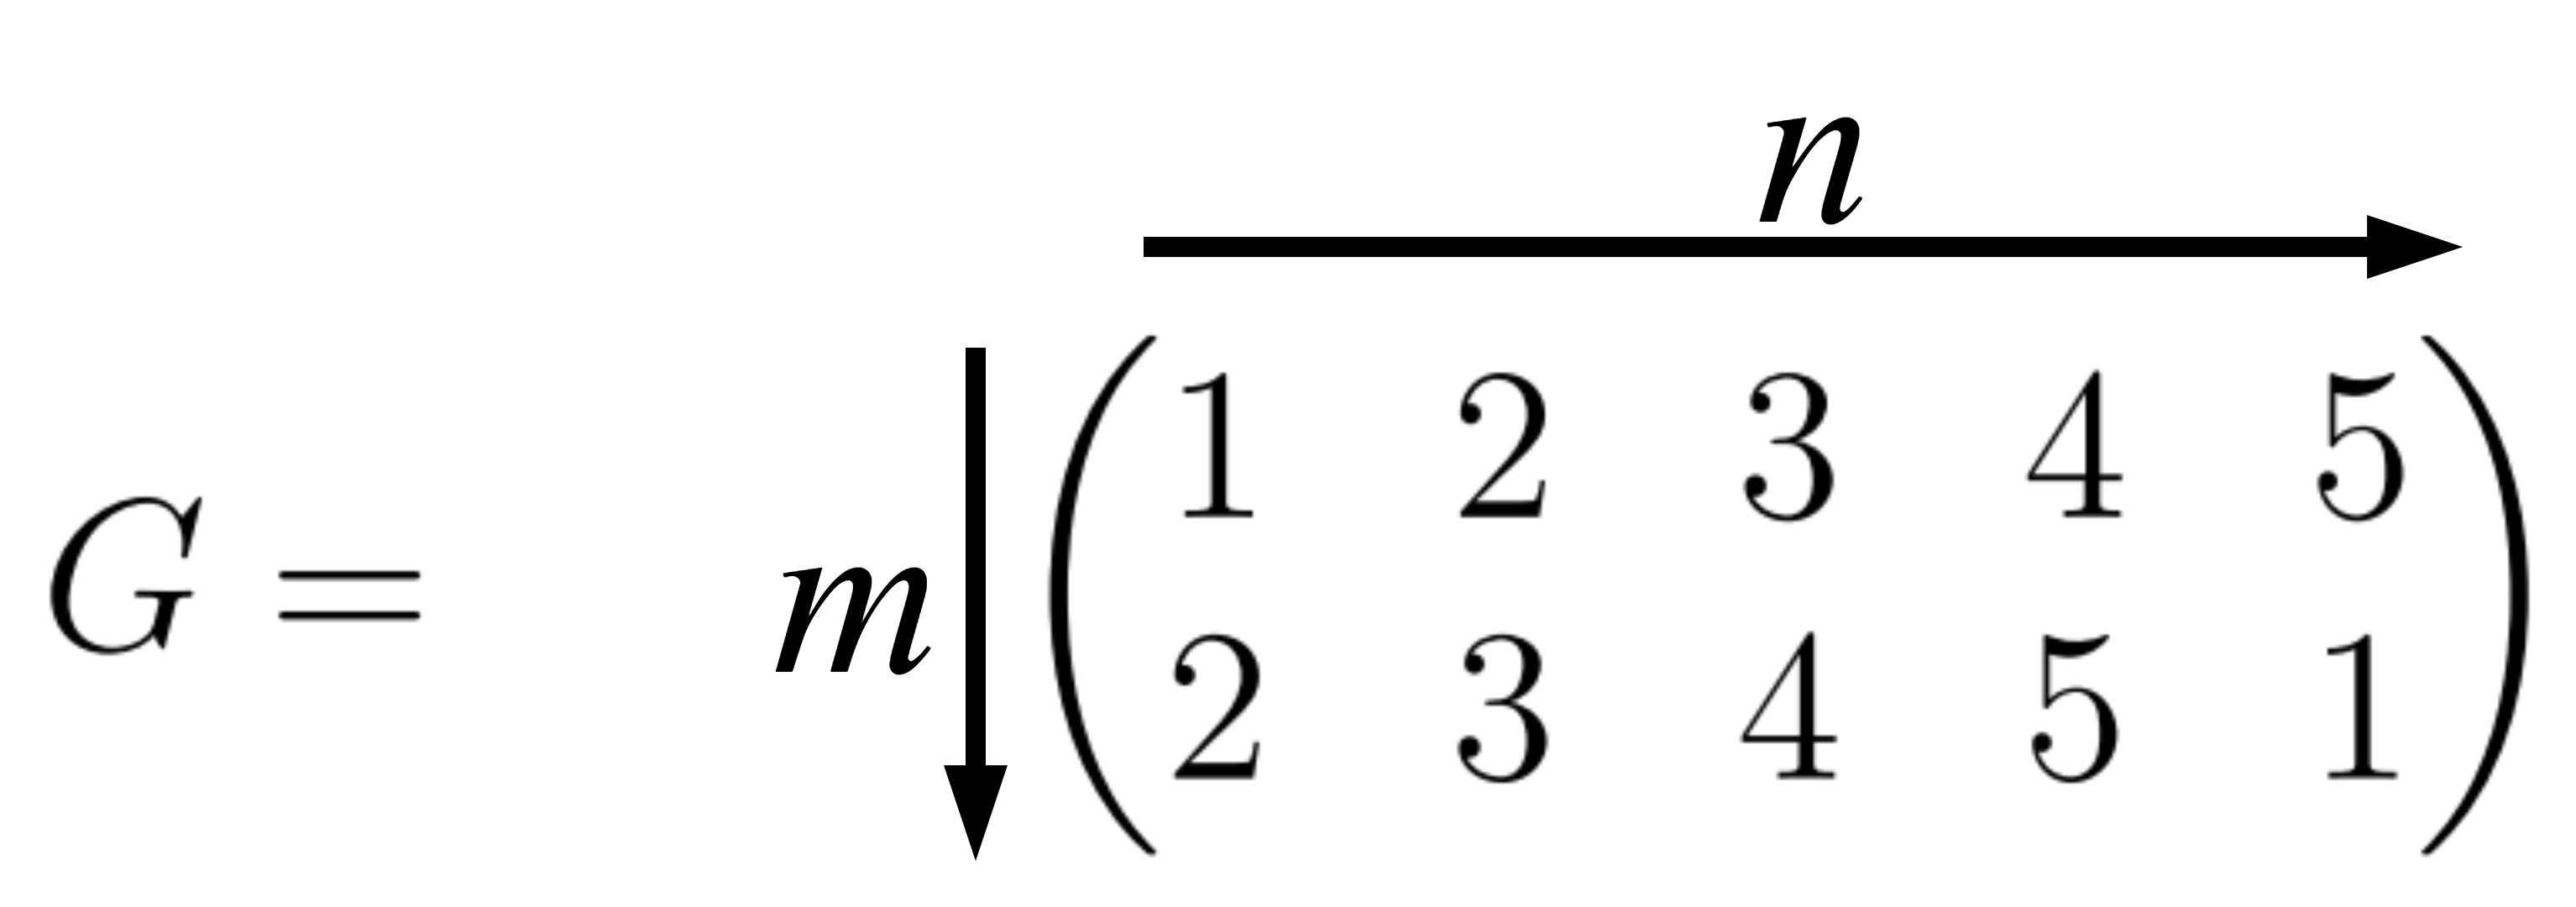
\includegraphics[width=0.6\textwidth]{graphics/generatormatrix.png}\\
\end{minipage}
\hfill
\begin{minipage}{0.5\textwidth}
\textbf{Aufbau Kontrollmatrix:}

\begin{itemize}
\item $(n \times n-m)$ Kontrollmatrix
\item Beispiel: $m= 2, n = 5$
\begin{itemize}
\item[$\rightarrow$] $(5 \times 5-2) = (5 \times 3)$ Kontrollmatrix
\end{itemize}
\end{itemize}\

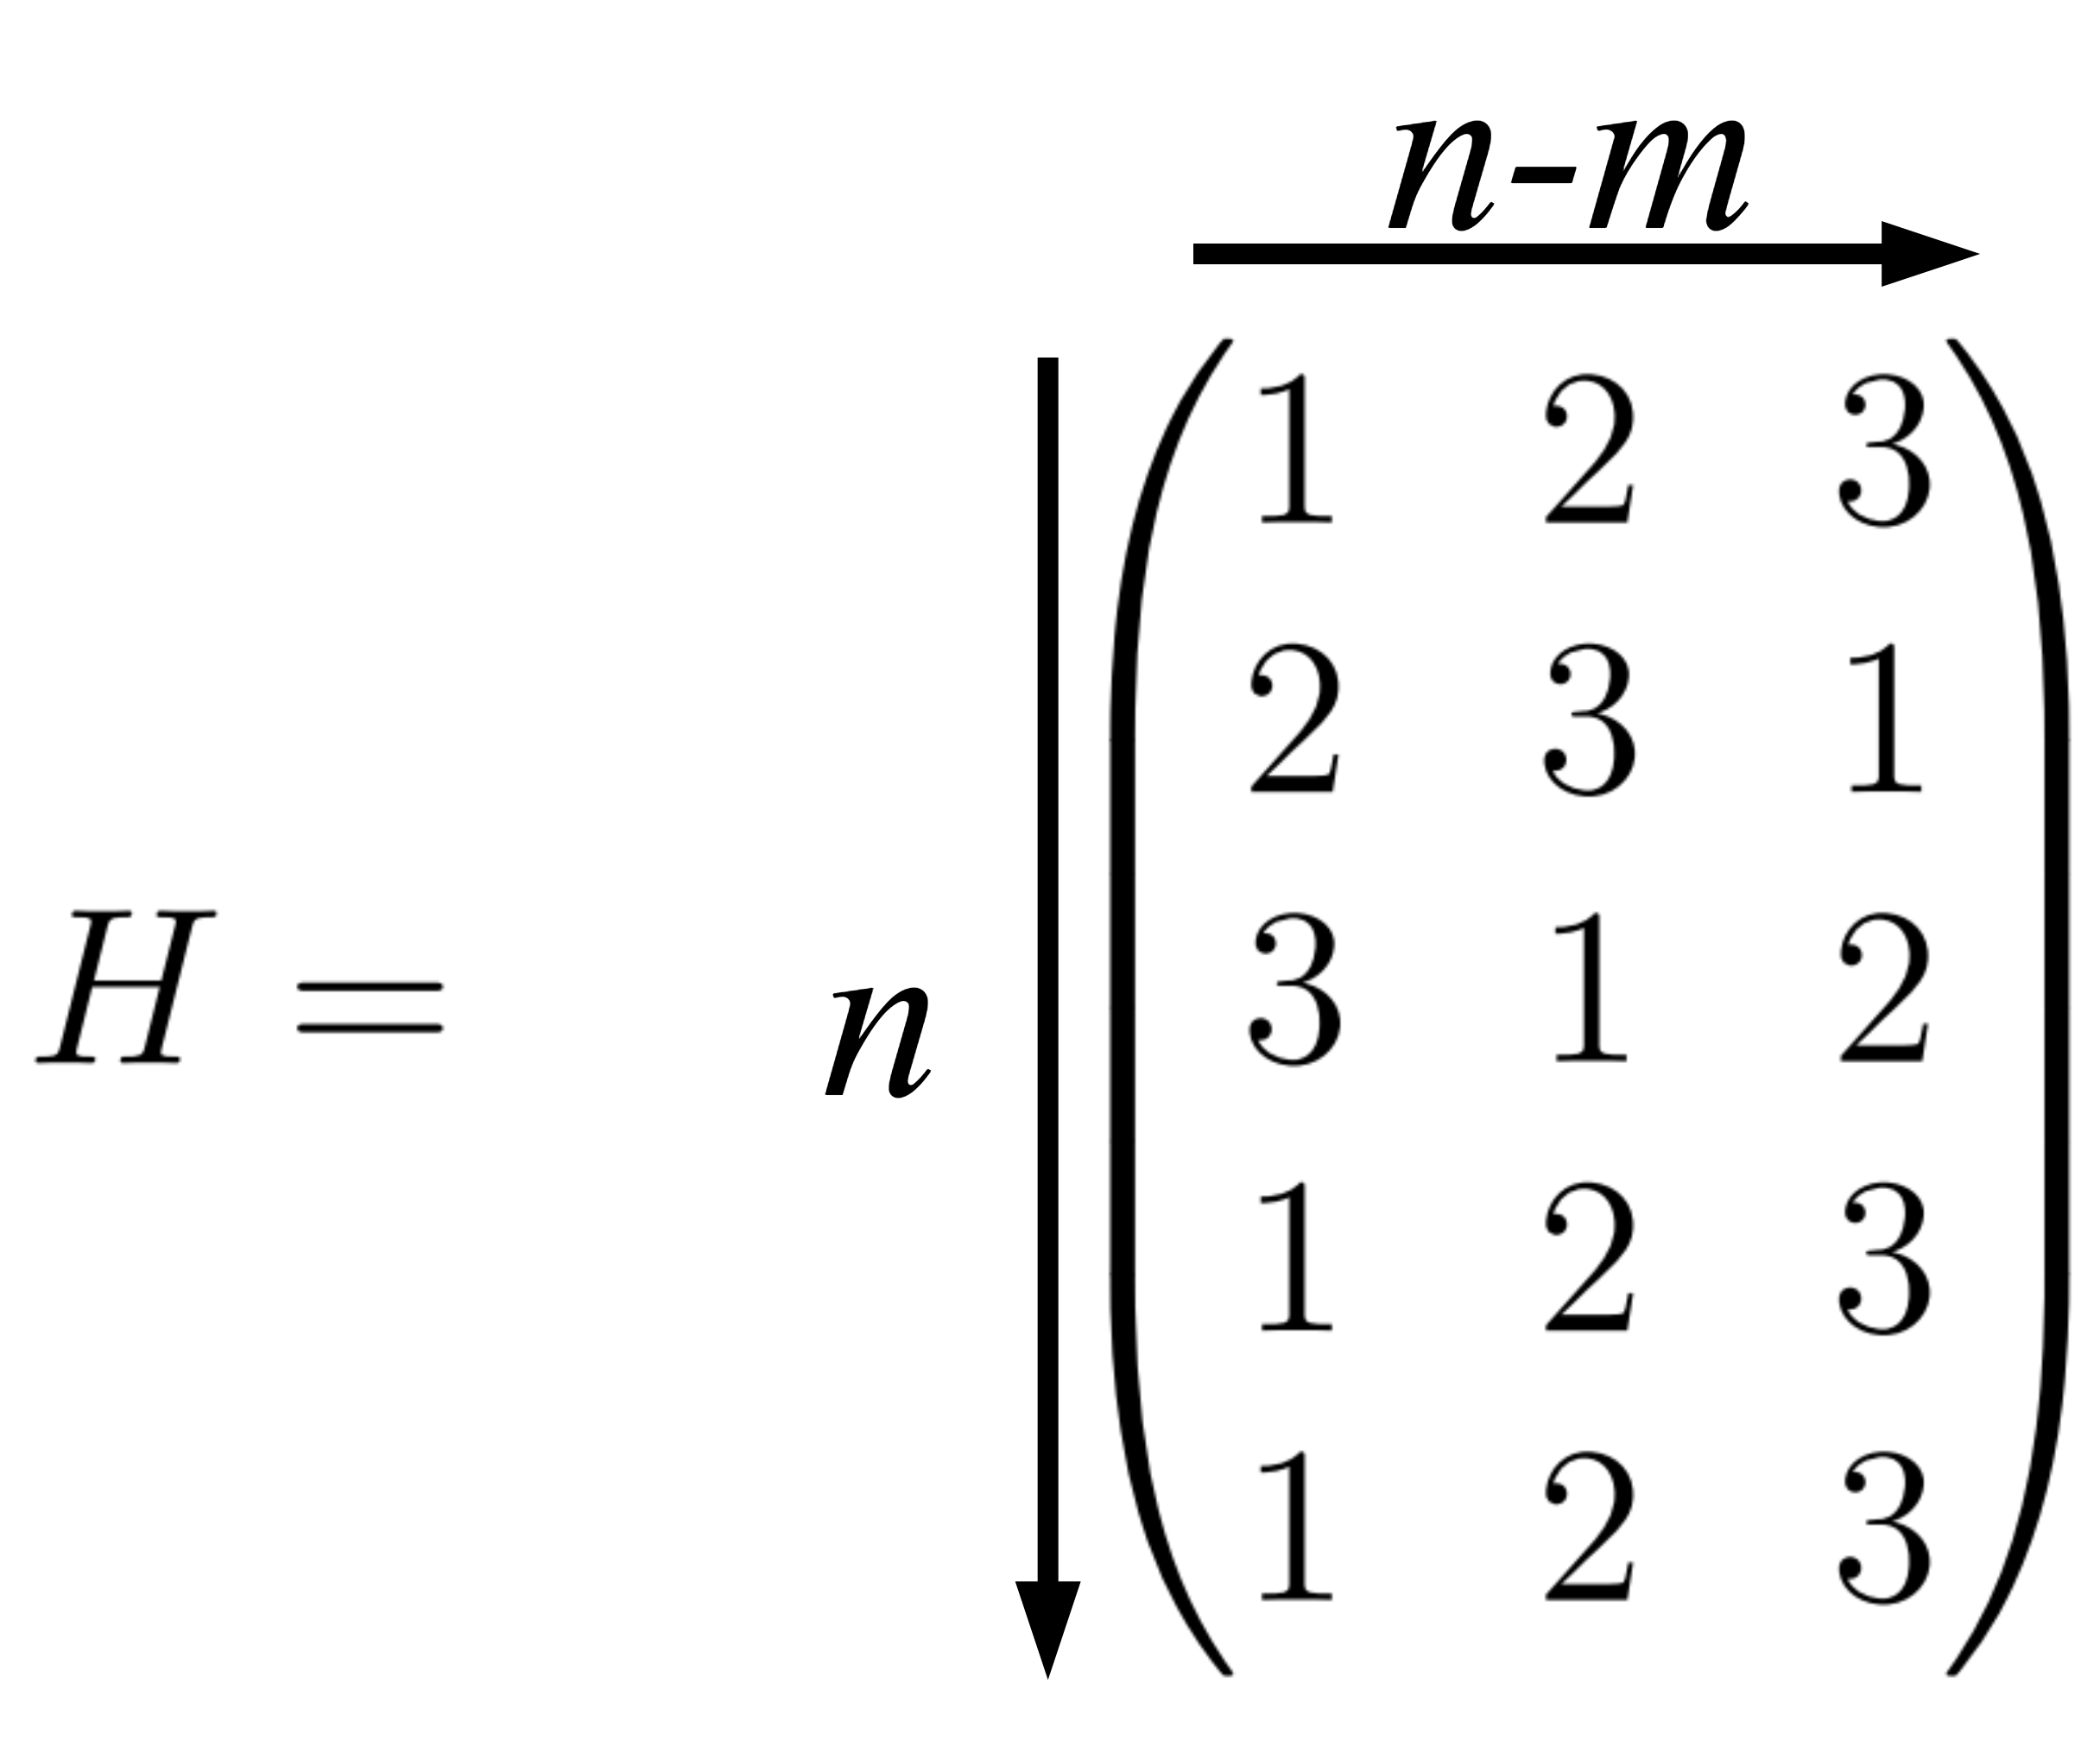
\includegraphics[width=0.5\textwidth]{graphics/kontrollmatrix.png}
\end{minipage}

\textbf{wort $\cdot$ matrix:}

$1010010 \cdot \begin{pmatrix}
1 & 1 & 1\\
1 & 0 & 1\\
0 & 1 & 1\\
1 & 1 & 0\\
1 & 0 & 0\\
0 & 1 & 0\\
0 & 0 & 1
\end{pmatrix} = \begin{pmatrix}
1\cdot1 & 1\cdot1 & 1\cdot1\\
1\cdot0 & 0\cdot0 & 1\cdot0\\
0\cdot1 & 1\cdot1 & 1\cdot1\\
1\cdot0 & 1\cdot0 & 0\cdot0\\
1\cdot0 & 0\cdot0 & 0\cdot0\\
0\cdot1 & 1\cdot1 & 0\cdot1\\
0\cdot0 & 0\cdot0 & 1\cdot0
\end{pmatrix} = \begin{pmatrix}
1 & 1 & 1\\
0 & 0 & 0\\
0 & 1 & 1\\
0 & 0 & 0\\
0 & 0 & 0\\
0 & 1 & 0\\
0 & 0 & 0
\end{pmatrix} = \begin{pmatrix}
\hspace{0.3cm}1 & | & \hspace{0.3cm}1 & | & \hspace{0.3cm}1\\
+0 & | & +0 & | & +0\\
+0 & | & +1 & | & +1\\
+0 & | & +0 & | & +0\\
+0 & | & +0 & | & +0\\
+0 & | & +1 & | & +0\\
+0 & \downarrow & +0 & \downarrow & +0
\end{pmatrix} = 110$\\~\\~\\

$1010010 \cdot \begin{pmatrix}
1 & 1 & 0 & 1 & 1 & 0 & 0\\
1 & 0 & 1 & 1 & 0 & 1 & 0\\
1 & 1 & 1 & 0 & 0 & 0 & 1
\end{pmatrix}^T = \begin{pmatrix}
1 \cdot 1 & 1 \cdot 0 & 0 \cdot 1 & 1 \cdot 0 & 1 \cdot 0 & 0 \cdot 1 & 0 \cdot 0\\
1 \cdot 1 & 0 \cdot 0 & 1 \cdot 1 & 1 \cdot 0 & 0 \cdot 0 & 1 \cdot 1 & 0 \cdot 0\\
1 \cdot 1 & 1 \cdot 0 & 1 \cdot 1 & 0 \cdot 0 & 0 \cdot 0 & 0 \cdot 1 & 1 \cdot 0
\end{pmatrix}^T =\\~\\~\\ \begin{pmatrix}
1 & 0 & 0 & 0 & 0 & 0 & 0\\
1 & 0 & 1 & 0 & 0 & 1 & 0\\
1 & 0 & 1 & 0 & 0 & 0 & 0
\end{pmatrix}^T = \begin{pmatrix}
1 & +0 & +0 & +0 & +0 & +0 & +0\\
- & - & - & - & - & - & \rightarrow\\
1 & +0 & +1 & +0 & +0 & +1 & +0\\
- & - & - & - & - & - & \rightarrow\\
1 & +0 & +1 & +0 & +0 & +0 & +0
\end{pmatrix}^T = 110$

\newpage

\subsection{Codewörter sind gegeben}

\subsubsection*{$n$ und $m$ bestimmen}

\begin{table}[h]
\centering
\begin{tabular}{c}
$n$ = Länge der Codewörter $\Rightarrow n = 5$\\
{\color{blue}00000}\\
01101\\
10111\\
11010\\
\end{tabular}
\end{table}

% === %

\begin{table}[h]
\centering
\begin{tabular}{c}
$m$ = Dimension $\Rightarrow m = 2$\\
{\color{blue}00}000\\
{\color{blue}01}101\\
{\color{blue}10}111\\
{\color{blue}11}010\\
\end{tabular}
\end{table}

\subsubsection*{Hamming-Distanz/Code-Distanz/$d(c)$}

\begin{itemize}
\item Hemming-Distanz ist die minimale Änderung des Gewichts
\item Wird mit $d(C)$ bezeichnet
\end{itemize}\

Beispiel:

\begin{itemize}
\item Anzahl Einsen in Codewörter Zählen
\item $0 \dots 0$ wird dabei nicht beachtet
\end{itemize}

\begin{table}[h]
\begin{tabular}{ccc}
01101 & $\rightarrow$ & Gewicht: 3\\
10111 & $\rightarrow$ & Gewicht: 4\\
11010 & $\rightarrow$ & Gewicht: 3\\
\end{tabular}
\end{table}

\begin{itemize}
\item Gewicht der Codewörter vergleichen und minimalstes auswählen
\item[$\Rightarrow$] $d(C) = 3$, da es minimal ist
\end{itemize}

\newpage

\subsubsection*{Kanonische Generatormatrix}

\begin{itemize}
\item Definition: Aus der Generatormatrix kann man alle möglichen Codewörter der Sprache erzeugen.
\item Falls die Generatormatrix gegeben ist, lässt sich die die kanonische Generatormatrix durch das Anwenden des Gaußschen Verfahrens auf die Generatormatrix erstellen.
\item Größe: $(m \times n)$
\item Aufbau: $G = \begin{pmatrix} E & G' \end{pmatrix}$
\begin{itemize}
\item ${\color{red}E}$: Einheitsmatrix
\item ${\color{ForestGreen}G'}$: Linear unabhängiger Rest aus Codewörtern
\end{itemize}

\end{itemize}

$$
G = \begin{pmatrix}
{\color{red}1} & {\color{red}0} & {\color{ForestGreen}1} & {\color{ForestGreen}1} & {\color{ForestGreen}1}\\
{\color{red}0} & {\color{red}1} & {\color{ForestGreen}1} & {\color{ForestGreen}0} & {\color{ForestGreen}1}
\end{pmatrix}
$$

\subsubsection*{Kanonische Kontrollmatrix}

\begin{itemize}
\item Definition: Erfüllt ein Wort $wort \cdot kontrollmatrix = 0$ ist es ein richtiges Codewort.
\item Größe: $n \times (n - m)$
\item Aufbau: $H = \begin{pmatrix}-G\\E\end{pmatrix}$
\begin{itemize}
\item ${\color{red}E}$: Einheitsmatrix
\item ${\color{ForestGreen}-G}$: Linear unabhängiger Rest aus Codewörtern
\end{itemize}
\end{itemize}

$$
H = \begin{pmatrix}
{\color{ForestGreen}-1} & {\color{ForestGreen}-1} & {\color{ForestGreen}-1}\\
{\color{ForestGreen}-1} & {\color{ForestGreen}-0} & {\color{ForestGreen}-1}\\
{\color{red}1} & {\color{red}0} & {\color{red}0}\\
{\color{red}0} & {\color{red}1} & {\color{red}0}\\
{\color{red}0} & {\color{red}0} & {\color{red}1}
\end{pmatrix} = \begin{pmatrix}
{\color{ForestGreen}1} & {\color{ForestGreen}1} & {\color{ForestGreen}1}\\
{\color{ForestGreen}1} & {\color{ForestGreen}0} & {\color{ForestGreen}1}\\
{\color{red}1} & {\color{red}0} & {\color{red}0}\\
{\color{red}0} & {\color{red}1} & {\color{red}0}\\
{\color{red}0} & {\color{red}0} & {\color{red}1}
\end{pmatrix}
$$

Modulo mit negativen Zahlen:

\begin{table}[h]
\begin{tabular}{c|cccccccccccccccccccc}
& $-10$ & $-9$ & $-8$ & $-7$ & $-6$ & $-5$ & $-4$ & $-3$ & $-2$ & $-1$ & $0$ & $1$ & $2$ & $3$ & $4$ & $5$ & $6$ & $7$ & $8$ & $9$\\
\hline
$\mathbb{Z}_2$ & & & & & & & & & $0$ & $1$ & $[0$ & $1]$ & & & & & & & &\\
\hline
$\mathbb{Z}_3$ & & & & & & & & $0$ & $1$ & $2$ & $[0$ & $1$ & $2]$ & & & & & & &\\
\hline
$\mathbb{Z}_4$ & & & & & & & $0$ & $1$ & $2$ & $3$ & $[0$ & $1$ & $2$ & $3]$ & & & & & &\\
\hline
$\mathbb{Z}_5$ & & & & & & $0$ & $1$ & $2$ & $3$ & $4$ & $[0$ & $1$ & $2$ & $3$ & $4]$ & & & & &\\
\hline
$\mathbb{Z}_6$ & & & & & $0$ & $1$ & $2$ & $3$ & $4$ & $5$ & $[0$ & $1$ & $2$ & $3$ & $4$ & $5]$ & & & &\\
\hline
$\mathbb{Z}_7$ & & & & $0$ & $1$ & $2$ & $3$ & $4$ & $5$ & $6$ & $[0$ & $1$ & $2$ & $3$ & $4$ & $5$ & $6]$ & & &\\
\hline
$\mathbb{Z}_8$ & & & $0$ & $1$ & $2$ & $3$ & $4$ & $5$ & $6$ & $7$ & $[0$ & $1$ & $2$ & $3$ & $4$ & $5$ & $6$ & $7]$ & &\\
\hline
$\mathbb{Z}_9$ & & $0$ & $1$ & $2$ & $3$ & $4$ & $5$ & $6$ & $7$ & $8$ & $[0$ & $1$ & $2$ & $3$ & $4$ & $5$ & $6$ & $7$ & $8]$ &\\
\hline
$\mathbb{Z}_{10}$ & $0$ & $1$ & $2$ & $3$ & $4$ & $5$ & $6$ & $7$ & $8$ & $9$ & $[0$ & $1$ & $2$ & $3$ & $4$ & $5$ & $6$ & $7$ & $8$ & $9]$\\
\end{tabular}
\end{table}

\newpage

\subsection{Syndromtabelle}

\begin{itemize}
\item Definition: Identifiziert und korrigiert Fehler in Codewörter durch Vergleich mit erwarteten Werten.
\item Anzahl Zeilen: $q^{n-m}$
\item Anzahl Spalten: $n$
\end{itemize}

Beispiel: $(7 \times 3)$-Kontrollmatrix, $n = 7, m = 4$

\begin{minipage}{0.2\textwidth}

$$
  H = \begin{pmatrix}
  {\color{red}1} & {\color{red}1} & {\color{red}1}\\
  {\color{blue}1} & {\color{blue}0} & {\color{blue}1}\\
  {\color{Green}0} & {\color{Green}1} & {\color{Green}1}\\
  1 & 1 & 0\\
  1 & 0 & 0\\
  0 & 1 & 0\\
  0 & 0 & 1
  \end{pmatrix}
$$
\end{minipage}
\hfill
\begin{minipage}{0.2\textwidth}

\begin{tabular}{c|c}
    $a$ & $S = a \cdot H$\\
    \hline
    0000000 & 000\\
    1000000 & {\color{red}111}\\
    0100000 & {\color{blue}101}\\
    0010000 & {\color{Green}011}\\
    0001000 & 110\\
    0000100 & 100\\
    0000010 & 010\\
    0000001 & 001\\
\end{tabular}
\end{minipage}
\hfill
\begin{minipage}{0.5\textwidth}

\begin{itemize}[leftmargin=*]
\item Anzahl Zeilen: $2^{7-4} = 8$
\item Anzahl Spalten: $7$
\item Wenn über $0000001$ hinaus geht egal ob $1000001$, $1100000$, \dots
\end{itemize}
\end{minipage}\

1. Überprüfen ob es ein empfangenes Codewort fehlerfrei ist$(wort \cdot kontrollmatrix = 0)$

\begin{itemize}
\item Empfangenes Wort: $y = 1010010$
\end{itemize}\

$1010010 \cdot \begin{pmatrix}
1 & 1 & 1\\
1 & 0 & 1\\
0 & 1 & 1\\
1 & 1 & 0\\
1 & 0 & 0\\
0 & 1 & 0\\
0 & 0 & 1
\end{pmatrix} = 110 \not = 0 \Rightarrow$ Fehler im empfangenen Codewort\\

2. Codewort durch Syndromtabelle korrigieren

\begin{itemize}
\item Klassenanführer von $110$ aus Syndromtabelle ablesen: $a =0001000$
\item $empfangenes \ Codewort - Klassenanfuehrer = korrigiertes \ Codewort$
\end{itemize}

\begin{table}[h]
\centering
\begin{tabular}{ccc}
$y$ & & $1010010$\\
$a$ & $-$ & $0001000$\\
\hline
& & $1011010$
\end{tabular}
\end{table}

\begin{itemize}
\item korrigiertes Codewort: $1011010$
\end{itemize}\

3. Nachricht extrahieren

\begin{itemize}
\item Letzte Stellen des korrigierten Codewort entfernen, um die Nachricht zu erhalten (Anzahl entfernte Stellen entspricht Länge des Syndrom).
\item Nachricht: 1011\sout{010} = 1011
\end{itemize}

\newpage

\subsection{Reed-Solomon-Codes}

\begin{itemize}
\item $RS(q,m,n)$
\item \textbf{Hamming-/Code-Distanz:} $d(C) = n - m + 1$
\item \textbf{Max. Anzahl Fehlerkorrigierend:} $\displaystyle \Bigl\lfloor \frac{(n - m)}{2} \Bigr\rfloor$
\item \textbf{Max. Anzahl Ausfällekorrigerend:} $(n - m)$
\end{itemize}\

\textbf{Nachricht codieren/Codewort erzeugen:}

\begin{itemize}
\item Da $q = 5$ alles $mod \ 5$
\item \textbf{Nachricht:} $a = ({\color{red}3}, {\color{red}4}, {\color{red}2})$
\item \textbf{Polynom:} $a(x) = a_0 + a_1x + a_2x^2 \xRightarrow[]{\text{\textit{a} einsetzen}} a(x) = {\color{red}3} + {\color{red}4}x + {\color{red}2}x^2$
\item \textbf{Stützstellen:} $u_1 = {\color{blue}0}, u_2 = {\color{Green}1}, u_3 = {\color{Orange}2}, u_4 = 3, u_5 = 4$
\end{itemize}\

$a(0) = 3 + 4\cdot {\color{blue}0} + 2\cdot {\color{blue}0^2} = 3$

$a(1) = 3 + 4\cdot {\color{Green}1} + 2\cdot {\color{Green}1^2} = 9 \ mod \ 5 = 4$

$a(2) = 3 + 4\cdot {\color{Orange}2} + 2\cdot {\color{Orange}2^2} = 19 \ mod \ 5 = 4$

$a(3) = 3 + 4\cdot 3 + 2\cdot 3^2 = 33 \ mod \ 5 = 3$

$a(4) = 3 + 4\cdot 4 + 2\cdot 4^2 = 51 \ mod \ 5 = 1$

$c(a) = (a(0),a(1),a(2),a(3),a(4)) = (3,4,4,3,1)$\\

\textbf{Ausfällekorrigieren: Fehlerhaftes Codewort bestimmen}

\begin{itemize}
\item Da $q = 5$ alles $mod \ 5$
\item \textbf{Fehlerhaftes Codewort:} $y = (3, *, 4, 3, *)$
\item \textbf{Polynom:} $a(x) = a_0 + a_1x + a_2x^2$
\item \textbf{Stützstellen:} $u_1 = 0, u_2 = 1, u_3 = 2, u_4 = 3, u_5 = 4$
\end{itemize}\

\begin{enumerate}[leftmargin=*]
\item Stützstellen und empfangenen (nicht fehlerhafte) Werte in das Polynom einsetzen um die Koeffizienten $a_0$, $a_1$, $a_2$ zu finden
\end{enumerate}

$a(0) = a_0 + a_1 \cdot 0 + a_2 \cdot 0^2 = 3 \Rightarrow \boxed{a_0 = 3}$

$a(2) = 3 + a_1 \cdot 2 + a_2 \cdot 2^2 = 4$\\
$\text{}\qquad = 3 + 2a_1 + 4a_2 = 4 \quad |-3 \ | -4a_2 \ | :2$\\
$\text{}\qquad = a_1 = \frac{1}{2} - 2a_2$

$a(3) = 3 + (\frac{1}{2} - 2a_2) \cdot 3 + a_2 \cdot 3^2 = 3$\\
$\text{}\qquad = 3 + 3(\frac{1}{2} - 2a_2) + 9a_2 = 3$\\
$\text{}\qquad = 3 + \frac{3}{2} - 6a_2 + 9a_2 = 3$\\
$\text{}\qquad = 4,5 + 3a_2 = 3 \quad |-4,5 \ | :3 \Rightarrow \boxed{a_1 = -\frac{1}{2}} \Rightarrow \boxed{a_2 = \frac{3}{2}}$\\

\begin{enumerate}[leftmargin=*, label={2.}]
\item Mit den gefunden Koeffizienten $a_0$, $a_1$, $a_2$ lassen sich nun die fehlenden Stellen herleiten
\end{enumerate}

$a(1) = 3 + \frac{3}{2} \cdot 1 - \frac{1}{2} \cdot 1^2 = \underline{\underline{4}}$

$a(4) = 3 + \frac{3}{2} \cdot 4 - \frac{1}{2} \cdot 4^2 = \underline{\underline{1}}$

Das Codewort ist somit $y = (3, 4, 4, 3, 1)$\\

\textbf{Generatormatrix erzeugen:}

\begin{itemize}
\item Beispiel: $m=3, n = 5, q = 5$
\item $u_1 = 0, u_2 = 1, u_3 = 2, u_4 = 3, u_5 = 4$
\end{itemize}\

$G = \begin{pmatrix}
1        & 1      & \dots & 1\\
u_1   & u_2    & \dots & u_n\\
u_1^2  & u_2^2  & \dots & u_n^2\\
u_1^3  & u_2^3  & \dots & u_n^3\\
\vdots & \vdots &  & \vdots\\
u_1^m  & u_2^m  & \dots & u_n^m
\end{pmatrix} = \begin{pmatrix}
1 & 1 & 1 & 1 & 1\\
0 & 1 & 2 & 3 & 4\\
0 & 1 & 2 & 9 & 16\\
0 & 1 & 8 & 27 & 64\\
\end{pmatrix}$\
\\

\textbf{Kontrollmatrix erzeugen:}

\begin{itemize}
\item Beispiel: $m=2, n = 5, q = 5$
\item $u_1 = 0, u_2 = 1, u_3 = 2, u_4 = 3, u_5 = 4$
\end{itemize}\

$H = \begin{pmatrix}
1 & 0 & 0 & \dots & 0\\
1 & 1 & 1 & \dots & 1\\
1 & u_3 & u_3^2 & \dots & u_3^{q-m-1}\\
1 & u_4 & u_4^2 & \dots & u_4^{q-m-1}\\
\vdots & \vdots & \vdots & & \vdots\\
1 & u_q & u_q^2 & \dots & u_q^{q-m-1}
\end{pmatrix} = \begin{pmatrix}
1 & 1 & 1\\
0 & 1 & 1\\
0 & 2 & 4\\
0 & 3 & 9\\
0 & 4 & 16
\end{pmatrix}$


\newpage

% =============================================

\section{Graphentheorie}

\subsection{Grundbegriffe}

$G(V,E)$, $V$ = Vertices = Knoten, $E$ = Edges = Kanten

\begin{minipage}{0.5\textwidth}
\subsubsection*{Gerichteter Graph}
\begin{itemize}[leftmargin=*]
\item Kante geht nur in \textit{eine} Richtung
\end{itemize}\
\\
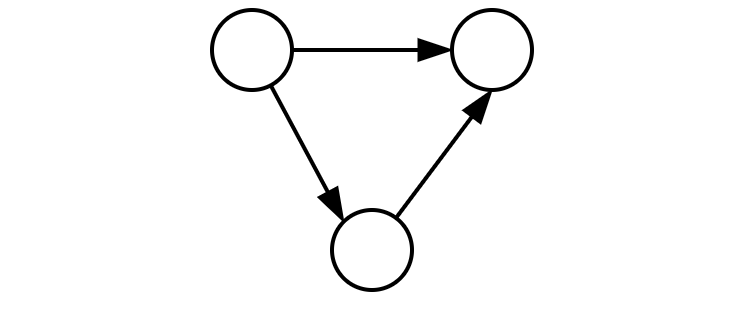
\includegraphics[width=0.6\textwidth]{graphics/graph_gerichtet.png}
\end{minipage}
\hfill
\begin{minipage}{0.5\textwidth}
\subsubsection*{Ungerichteter Graph}
\begin{itemize}[leftmargin=*]
\item Kante geht nur in \textit{beide} Richtung
\end{itemize}\
\\
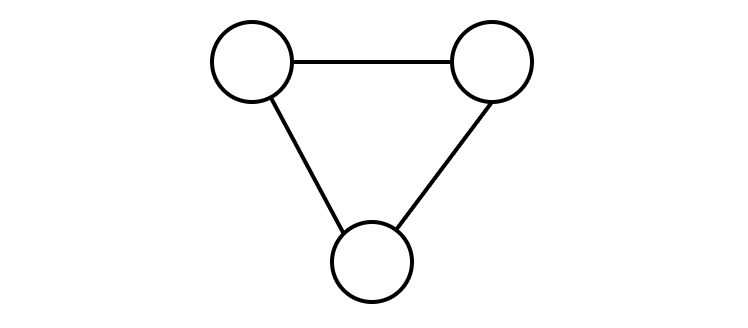
\includegraphics[width=0.6\textwidth]{graphics/graph_ungerichtet.png}
\end{minipage}


\begin{minipage}{0.5\textwidth}
\subsubsection*{Zusammenhängender Graph}
\begin{itemize}[leftmargin=*]
\item Verbindung von einem Knotenpunkt zu allen anderen
\item Verbindungen müssen nicht direkt sein
\item Gibt keine isolierten Knoten
\end{itemize}\
\\
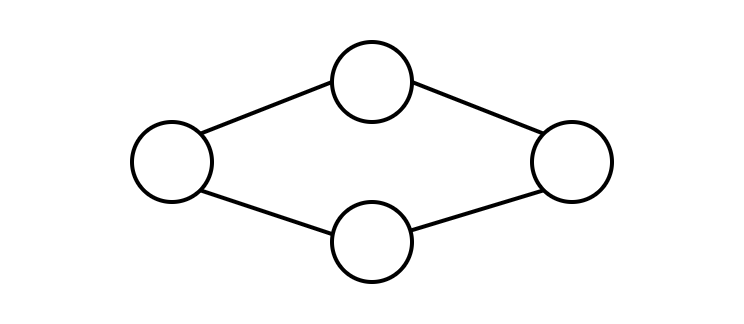
\includegraphics[width=0.6\textwidth]{graphics/graph_zusammen.png}
\end{minipage}
\hfill
\begin{minipage}{0.5\textwidth}
\subsubsection*{Nichtzusammenhängender Graph}
\begin{itemize}[leftmargin=*]
\item Wenn ein Knoten isoliert ist und keine Verbindung herrscht
\end{itemize}\
\\
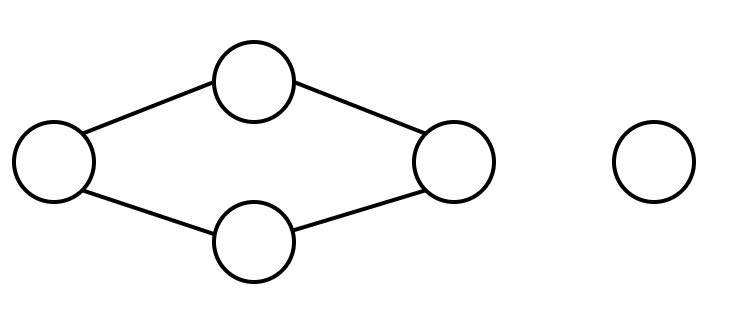
\includegraphics[width=0.6\textwidth]{graphics/graph_nicht_zusammen.png}
\end{minipage}

\begin{minipage}{0.5\textwidth}
\subsubsection*{Gewichteter Graph}
\begin{itemize}[leftmargin=*]
\item Die Kanten bekommen Gewichte zugewiesen
\end{itemize}\
\\
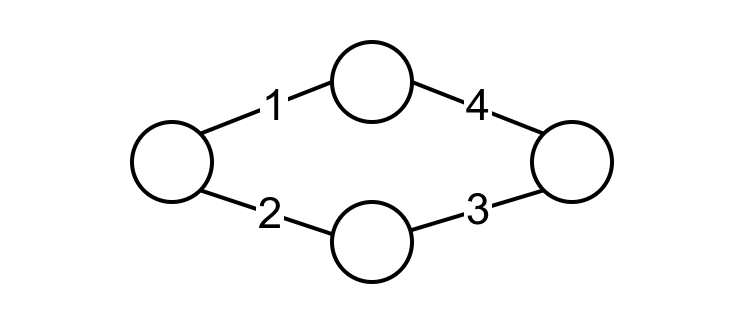
\includegraphics[width=0.6\textwidth]{graphics/graph_gewicht.png}
\end{minipage}
\hfill
\begin{minipage}{0.5\textwidth}
\subsubsection*{Knotengrad}
\begin{itemize}[leftmargin=*]
\item Anzahl Kanten die von einem Knoten ausgehen
\end{itemize}\
\\
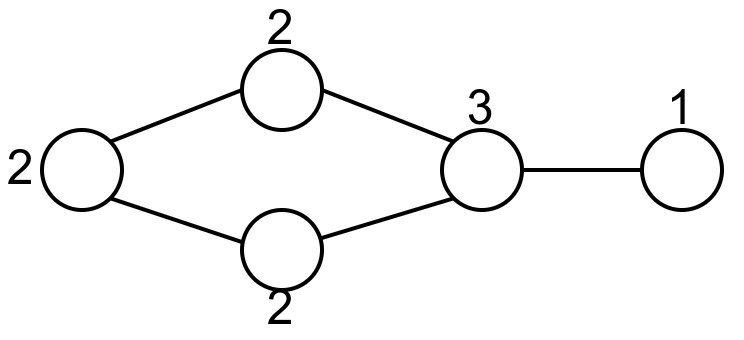
\includegraphics[width=0.6\textwidth]{graphics/graph_knotengrad.png}
\end{minipage}

\begin{minipage}{0.5\textwidth}
\subsubsection*{Euler-Zyklus/Eulersch}
\begin{itemize}[leftmargin=*]
\item Anfangszustand = Endzustand
\item Alle Knoten haben einen geraden Grad
\end{itemize}\
\\
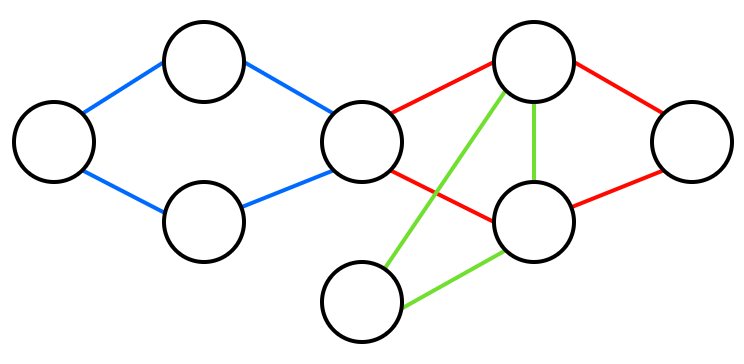
\includegraphics[width=0.6\textwidth]{graphics/graph_euler_zyklus.png}
\end{minipage}
\hfill
\begin{minipage}{0.5\textwidth}
\subsubsection*{Euler-Pfad}
\begin{itemize}[leftmargin=*]
\item Jede Kante wird genau einmal durchlaufen
\item Keine Kante wird mehrmals durchlaufen
\item Startknoten muss nicht gleich Endknoten sein
\item Genau zwei Knoten haben einen ungeraden Grad
\end{itemize}\
\\
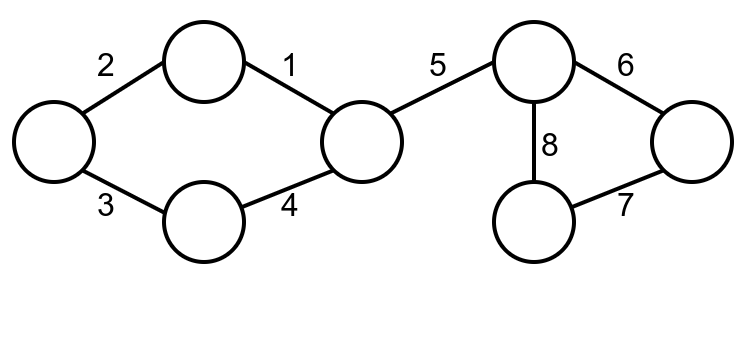
\includegraphics[width=0.6\textwidth]{graphics/graph_euler_pfad.png}\end{minipage}

\newpage

\begin{minipage}{0.5\textwidth}
\subsubsection*{Hamilton-Zyklus}
\begin{itemize}[leftmargin=*]
\item Anfangszustand = Endzustand
\item Alle Knoten geraden Grads
\end{itemize}\
\\
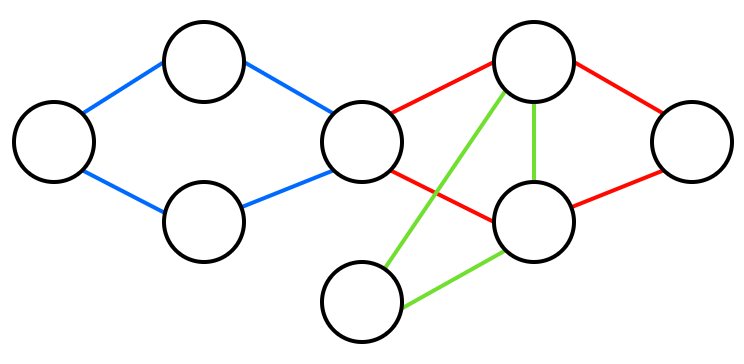
\includegraphics[width=0.6\textwidth]{graphics/graph_euler_zyklus.png}
\end{minipage}
\hfill
\begin{minipage}{0.5\textwidth}
\subsubsection*{Hamilton-Pfad}
\begin{itemize}[leftmargin=*]
\item Jede Kante wird genau einmal durchlaufen
\item Keine Kante wird mehrmals durchlaufen
\item Startknoten muss nicht gleich Endknoten sein
\end{itemize}\
\\
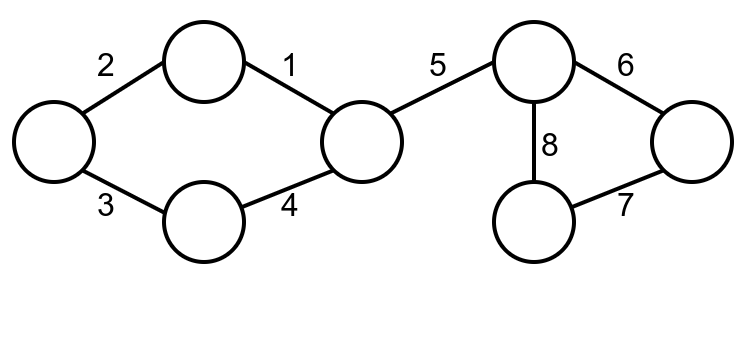
\includegraphics[width=0.6\textwidth]{graphics/graph_euler_pfad.png}\end{minipage}

\subsubsection*{Bipartit}

\begin{itemize}
\item Man kann alle Knoten in zwei (disjunkte) Teilmengen/Gruppen aufteilen
\item Jede Verbindung geht dabei von einer Teilmenge/Gruppe in die andere
\item Es darf allerdings keine Verbindung der Knoten innerhalb der eigenen Teilmenge/Gruppe geben
\end{itemize}

\begin{figure}[h]
\centering
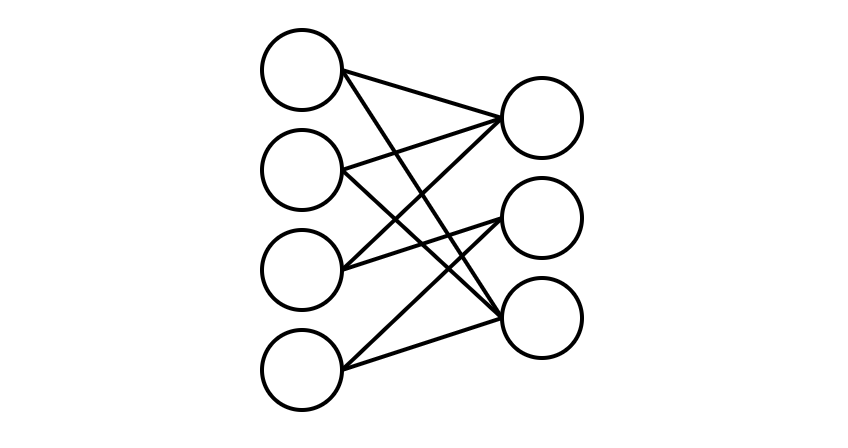
\includegraphics[width=0.4\textwidth]{graphics/graph_bipartit.png}
\end{figure}

\textbf{Beispiel:} Zeigen ob ein Graph bipartit ist

\begin{itemize}
\item Beliebigen Knoten auswählen und färben (z.B blau).
\item Alle benachbarte Knoten mit einer anderen Farbe färben (z.B grün)
\item Widerholen: Alle Knoten die an einen blauen Knoten angrenzen, grün und alle Knoten, die an einen grünen Knoten angrenzen, blau färben.
\item Prüfung: Wenn man auf einen Knoten stößt, der bereits gefärbt ist und dessen Farbe sich von der Farbe unterscheidet, die man ihm zuweisen möchten, dann ist der Graph \textit{nicht bipartit}. Wenn man alle Knoten ohne solche Konflikte färben konnte, ist der Graph \textit{bipartit}.
\item Die blauen Knoten sind am Ende die eine Teilmenge/Gruppe und die grünen Knoten sind am Ende die andere Teilmenge/Gruppe
\end{itemize}

\begin{figure}[h]
\centering
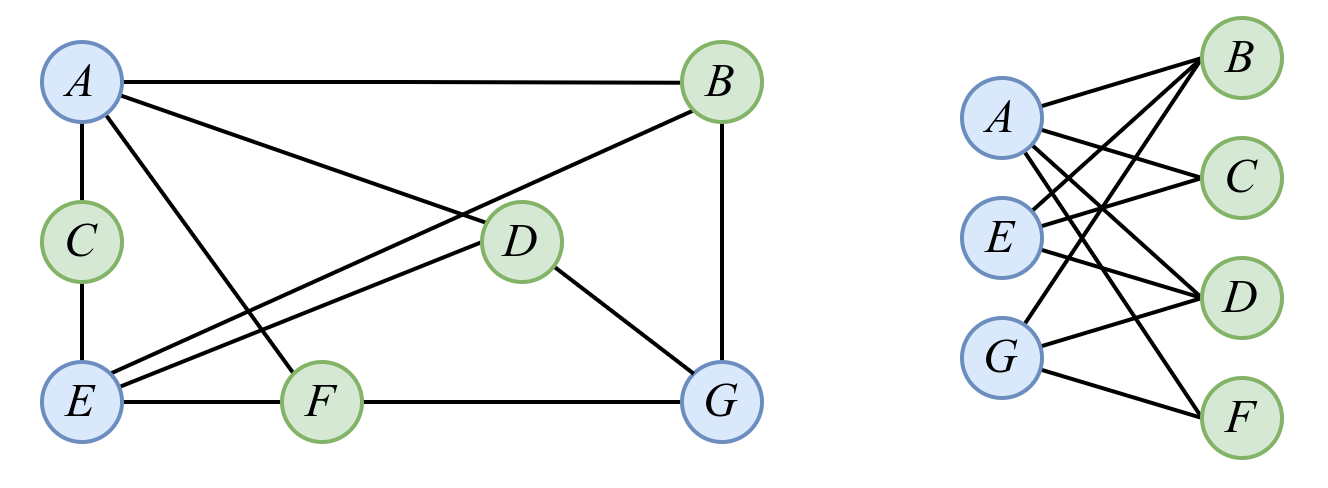
\includegraphics[width=0.75\textwidth]{graphics/graph_bipartit2.png}
\end{figure}

\newpage

\subsubsection*{Planar}

\begin{itemize}
\item Ein Graph ist planar, wenn man ihn so zeichnen kann, dass sich seine Kanten nirgendwo kreuzen.
\end{itemize}\

\textbf{(Nicht) Planarität prüfen:}

\textbf{1 Methode:}

\begin{itemize}
\item $n = |V|$ (Anzahl Knoten) und $m = |E|$ (Anzahl Kanten) bestimmen
\item Hat der Graph einen Zyklus der Länge 3?
	\begin{itemize}
	\item[$\rightarrow$] \textbf{Ja:} $m \leq 3n - 6$
	\item[$\rightarrow$] \textbf{Nein:} $m \leq 2n - 4$
	\item Gilt $m \not \leq 3n - 6$ oder $m \not \leq 2n - 4$ ist der Graph \textit{nicht planar}
	\item \textbf{Achtung:} Die Formel macht nur eine Aussage darüber, ob der Graph nicht planar ist, aber nicht, ob ein Graph planar ist. Gilt also $m \leq 3n - 6$ oder $m \leq 2n - 4$ heißt es nicht, dass der Graph planar ist. Man kann also nur die Nichtplanarität überprüfen.
	\end{itemize}
\end{itemize}

\textbf{2 Methode:}

\begin{itemize}
\item Ist der $K_5$ oder $K_{3,3}$ der Graph oder ein Teilgraph ist der ein Graph immer \textit{nicht planar}
\end{itemize}

\begin{figure}[h]
\centering
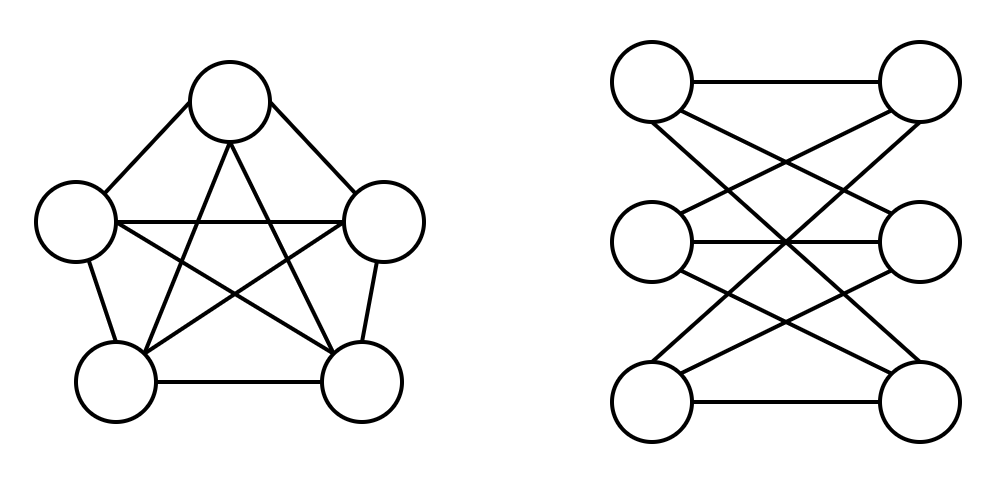
\includegraphics[width=0.4\textwidth]{graphics/graph_planar.png}
\caption*{$K_5$ (links), $K_{3,3}$ (rechts)}
\end{figure}

\textbf{3 Methode:}

\begin{itemize}
\item Graphen versuchen so zu zeichnen das ein planarer Graph rauskommt (umständlich)
\end{itemize}

\newpage

\subsection{Kürzester Weg}

\subsubsection*{Dijkstra}

\begin{figure}[h]
\centering
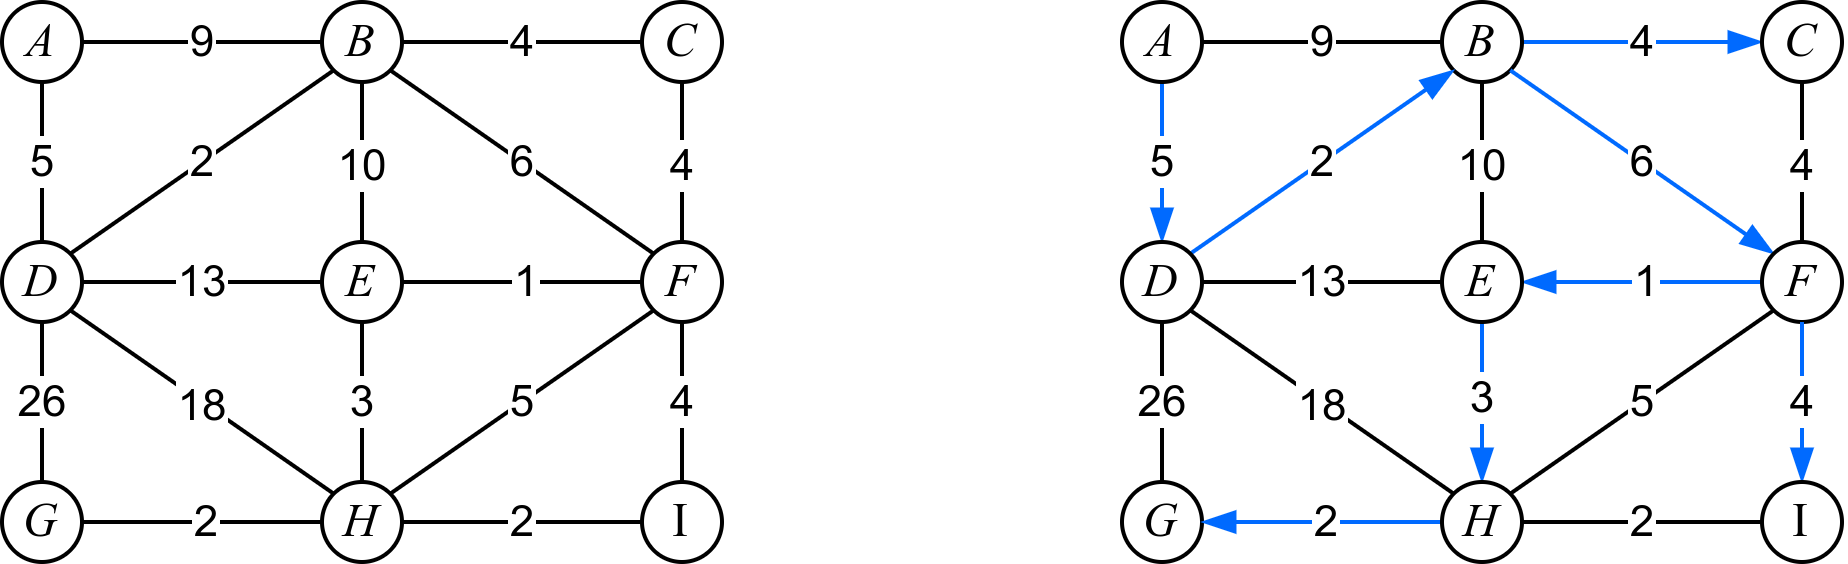
\includegraphics[width=0.9\textwidth]{graphics/dijkstra.png}
\end{figure}

\begin{table}[h]
\centering
\begin{tabular}{c|c|c|c|c|c|c|c|c||l}
A & B & C & D & E & F & G & H & I & S\\
\hline
0(A) &      & & & & & & & & A\\
0(A) & 9(A) &       & 5(D) & & & & & & A, D\\
0(A) & 7(D) &       & 5(D) & 18(E) & & 31(D) & 23(D) & & A, D, B\\
0(A) & 7(D) & 11(B) & 5(D) & 17(E) & 13(B) & 31(D) & 23(D) & & A, D, B, C\\
0(A) & 7(D) & 11(B) & 5(D) & 17(E) & 13(B) & 31(D) & 23(D) & & A, D, B, C, F\\
0(A) & 7(D) & 11(B) & 5(D) & 14(F) & 13(B) & 31(D) & 18(F) & 17(F) & A, D, B, C, F, E\\
0(A) & 7(D) & 11(B) & 5(D) & 14(F) & 13(B) & 31(D) & 17(E) & 17(F) & A, D, B, C, F, E, H\\
0(A) & 7(D) & 11(B) & 5(D) & 14(F) & 13(B) & 31(D) & 17(E) & 17(F) & A, D, B, C, F, E, H, I\\
0(A) & 7(D) & 11(B) & 5(D) & 14(F) & 13(B) & 31(D) & 17(E) & 17(F) & A, D, B, C, F, E, H, I, G
\end{tabular}
\end{table}

\newpage

\subsubsection*{Floyd}

\begin{figure}[h]
\centering
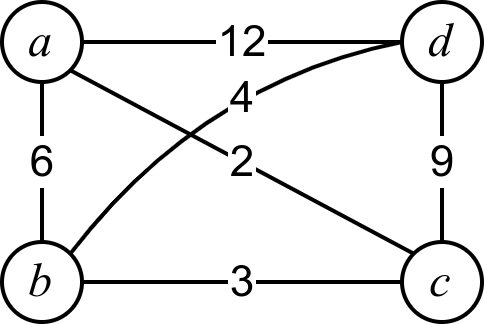
\includegraphics[width=0.3\textwidth]{graphics/floyd.png}
\end{figure}

\begin{table}[h]
\centering
\begin{tabular}{c|c|cccc|cccc}
& $i$ & $a$ & $b$ & $c$ & $d$ & $a$ & $b$ & $c$ & $d$\\
\hline
& $a$ & 0  & 6 & 2 & 12 & $a$ & $a$ & $a$ & $a$\\ 
& $b$ & 6  & 0 & 3 & 4  & $b$ & $b$ & $b$ & $b$\\
& $c$ & 2  & 3 & 0 & 9  & $c$ & $c$ & $c$ & $c$\\
& $d$ & 12 & 4 & 9 & 0  & $d$ & $d$ & $d$ & $d$\\
\hline
1 & $a$ & {\color{red}0}  & {\color{red}6} & {\color{red}2} & {\color{red}12} & {\color{red}$a$} & {\color{red}$a$} & {\color{red}$a$} & {\color{red}$a$}\\ 
1 & $b$ & {\color{red}6}  & 0 & 3 & 4  & $b$ & $b$ & $b$ & $b$\\
1 & $c$ & {\color{red}2}  & 3 & 0 & 9  & $c$ & $c$ & $c$ & $c$\\
1 & $d$ & {\color{red}12} & 4 & 9 & 0  & $d$ & $d$ & $d$ & $d$\\
\hline
2 & $a$ & 0  & {\color{red}6} & 2 & {\color{blue}10} & $a$ & $a$ & $a$ & {\color{blue}$b$}\\ 
2 & $b$ & {\color{red}6}  & {\color{red}0} & {\color{red}3} & {\color{red}4} & {\color{red}$b$} & {\color{red}$b$} & {\color{red}$b$} & {\color{red}$b$}\\
2 & $c$ & 2  & {\color{red}3} & 0 & {\color{blue}7}  & $c$ & $c$ & $c$ & {\color{blue}$b$}\\
2 & $d$ & {\color{blue}10} & {\color{red}4} & {\color{blue}7} & 0  & {\color{blue}$b$} & $d$ & {\color{blue}$b$} & $d$\\
\hline
3 & $a$ & 0  & {\color{blue}5} & {\color{red}2} & {\color{blue}9} & $a$ & {\color{blue}$c$} & $a$ & $b$\\
3 & $b$ & {\color{blue}5}  & 0 & {\color{red}3} & 4  & {\color{blue}c} & $b$ & $b$ & $b$\\
3 & $c$ & {\color{red}2}  & {\color{red}3} & {\color{red}0} & {\color{red}7}  & {\color{red}$c$} & {\color{red}$c$} & {\color{red}$c$} & {\color{red}$b$}\\
3 & $d$ & {\color{blue}9} & 4 & {\color{red}7} & 0  & {\color{blue}c} & $d$ & $b$ & $d$\\
\hline
4 & $a$ & 0 & 5 & 2 & {\color{red}9} & $a$ & $c$ & $a$ & $b$\\ 
4 & $b$ & 5 & 0 & 3 & {\color{red}4} & $c$ & $b$ & $b$ & $b$\\
4 & $c$ & 2 & 3 & 0 & {\color{red}7} & $c$ & $c$ & $c$ & $b$\\
4 & $d$ & {\color{red}9} & {\color{red}4} & {\color{red}7} & {\color{red}0} & {\color{red}$c$} & {\color{red}$d$} & {\color{red}$b$} & {\color{red}$d$}\\
\end{tabular}
\end{table}

\newpage

\subsubsection*{FIFO}

\begin{figure}[h]
\centering
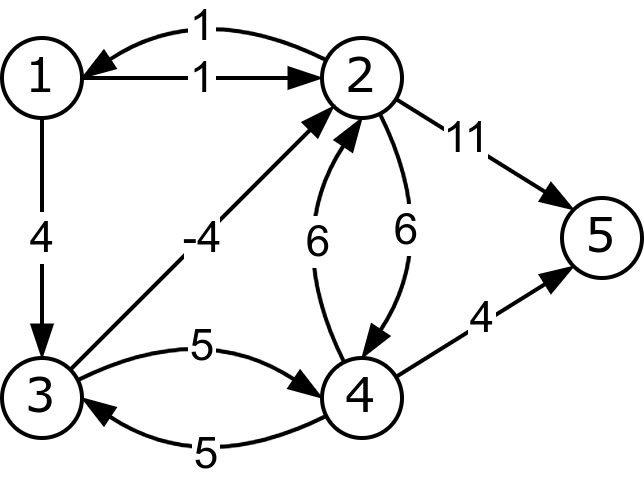
\includegraphics[width=0.35\textwidth]{graphics/fifo.png}
\end{figure}

\begin{table}[h]
\centering
\begin{tabular}{c|c|c|c|c||c|c|c|c|c||l}
D(s,1) & D(s,2) & D(s,3) & D(s,4) & D(s,5) & R(1) & R(2) & R(3) & R(4) & R(5) & S\\
\hline
0 &   &   &   &    & &   &   &   &   & $1$\\
0 & 1 & 4 &   &    & & 1 & 1 &   &   & $2 < 3$\\
0 & 1 & 4 & 7 & 12 & & 1 & 1 & 2 & 2 & $3 < 4 < 5$\\
0 & 0 & 4 & 7 & 12 & & 3 & 1 & 2 & 2 & $4 < 5 < 2$\\
0 & 0 & 4 & 6 & 11 & & 3 & 1 & 2 & 4 & $5 < 2$\\
0 & 0 & 4 & 6 & 11 & & 3 & 1 & 2 & 4 & $2$\\
0 & 0 & 4 & 6 & 10 & & 3 & 1 & 2 & 4 & $4$\\
0 & 0 & 4 & 6 & 10 & & 3 & 1 & 2 & 4 & $5$\\
0 & 0 & 4 & 6 & 10 & & 3 & 1 & 2 & 4 &
\end{tabular}
\end{table}


% =============================================

\end{document}

